\documentclass[aps,pra,twocolumn,amsmath,amssymb,nofootinbib,superscriptaddress]{revtex4}

\newcommand{\bra}[1]{\langle#1|}
\newcommand{\ket}[1]{|#1\rangle}
\newcommand{\op}[2]{\hat{\textbf{#1}}_{#2}}
\newcommand{\dagop}[2]{\hat{\textbf{#1}}_{#2}^\dag}
\usepackage[pdftex]{graphicx}
\usepackage{mathrsfs}
\usepackage[colorlinks]{hyperref}

\begin{document}

\bibliographystyle{apsrev}

\title{Notes on fidelity in boson-sampling (for Chaoyang's group)}

\frenchspacing

\maketitle

\begin{figure}[!htb]
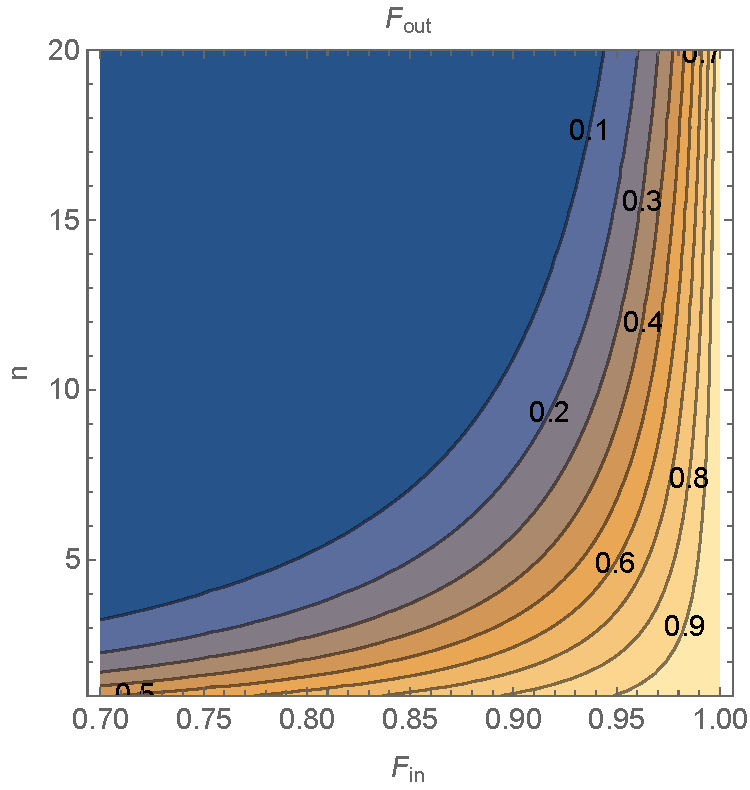
\includegraphics[width=\columnwidth]{fidelity}
\caption{Fidelity of the output state of a boson-sampler, $F_\mathrm{out}$, given single-photon input fidelities of $F_\mathrm{in}$, where $n$ is the number of photons entering the circuit.} \label{fig:fidelity}
\end{figure}

Ordinarily, we represent photons as the photon creation operator acting on the vacuum state, \mbox{$\ket{1}=\hat{a}^\dag\ket{0}$}. This is appropriate when dealing with indistinguishable photons. However, photons have rich spatio-temporal structure, and in these degrees of freedom photons are never perfectly indistinguishable. To capture this, we replace photon creation operators with mode operators, that represent photons in these additional degrees of freedom,
\begin{align}
\hat{A}^\dag_\psi = \int_{-\infty}^\infty \psi(t) \hat{a}^\dag(t) \,dt.
\end{align}
Here $\psi$ is the temporal distribution function (TDF) of the photon, and $\hat{a}^\dag(t)$ is the time-specific creation operator. $\psi$ is normalised, such that,
\begin{align}
\int_{-\infty}^\infty |\psi(t)|^2 \, dt = 1.
\end{align}
The Fourier transform gives us the spectral distribution function. Then, a single-photon state with associated TDF $\psi$, is given by,
\begin{align}
\ket{1_\psi} = \hat{A}^\dag_\psi \ket{0}.
\end{align}
This can be logically generalised into other degrees of freedom, such as the spatial degrees of freedom. For example, to capture both temporal and x-y spatial degrees of freedom, we could use the representation,
\begin{align}
\hat{A}^\dag_\psi = \int_{-\infty}^\infty \int_{-\infty}^\infty \int_{-\infty}^\infty \psi(t,x,y) \hat{a}^\dag(t,x,y) \, dt\, dx\, dy.
\end{align}

The overlap of two single-photon states characterised by distinct TDFs is simply,
\begin{align}
\langle 1_\psi | 1_\phi \rangle &= \bra{0} \hat{A}_{\psi} \hat{A}^\dag_{\phi} \ket{0} \nonumber \\
&= \int_{-\infty}^\infty \int_{-\infty}^\infty \psi(t)^*\phi(t') \langle t|t'\rangle \, dt \, dt' \nonumber \\
&= \int_{-\infty}^\infty \int_{-\infty}^\infty \psi(t)^*\phi(t') \delta(t-t')\,dt \, dt' \nonumber \\
&= \int_{-\infty}^\infty \psi(t)^*\phi(t) \,dt.
\end{align}

If we choose an orthonormal basis of TDFs, an arbitrary photon may be decomposed into a linear combination of the associated basis mode operators. Let us define such a basis as $\{\xi\}$. Let $\xi_0$ be the `desired' spatio-temporal mode. Because of the orthonormality,
\begin{align}
\bra{0} \hat{A}_{\xi_i} \hat{A}^\dag_{\xi_j} \ket{0} = \delta_{i,j},
\end{align}
we define our mode operators as,
\begin{align}
\hat{A}^\dag_{\psi_i} = \alpha \hat{A}^\dag_{\xi_0} + \sqrt{1-\alpha^2} \hat{A}^\dag_{\xi_i}.
\end{align}
That is, each input photon has an amplitude overlap of $\alpha$ with every other, via the $\xi_0$ component of the TDF.

Exactly the same argument applies to incoherent processes, such as time-jitter, except that rather than being a coherent superposition of different spatio-temporal modes, the density operator would be a classical mixture of the different terms,

Then the fidelity of a single-photon input is,
\begin{align}
F_\mathrm{in} = |\alpha|^2.
\end{align}
The fidelity of the entire $n$-photon input state is then,
\begin{align}
F_\mathrm{total} &= {F_\mathrm{in}}^n \nonumber \\
&= |\alpha|^{2n}.
\end{align}
This can be interpreted as the probability that, upon measurement, we have projected onto the desired spatio-temporal mode.

Since the fidelity between two states is invariant under a common unitary evolution,
\begin{align}
F(\ket\psi,\ket\phi) = F(\hat{U}\ket\psi, \hat{U}\ket\phi),
\end{align}
the output fidelity is the same as the input fidelity, \mbox{$F_\mathrm{out} = F_\mathrm{total}$}.

The relationship between the single-photon input and net output fidelities are illustrated in Fig.~\ref{fig:fidelity}. Based on this, to achieve an output fidelity of \mbox{$F_\mathrm{out} = 0.9$} requires single-photon input fidelities of \mbox{$F_\mathrm{in} = 0.995$} for 10 photons, and \mbox{$F_\mathrm{in} = 0.998$} for 20 photons. This type of single-photon interference fidelity is realistic using present-day technology, which comes very close to unity.

\end{document}
